\clearpage
\subsection{実習3-1 固定抵抗の電圧電流特性}
\begin{itemize}
	\item プログラム\ref{ex31-block}は$R_{0}$の場合の,固定抵抗の電圧電流特性(0-5\,\rm{V}まで0.1\,\rm{V}刻み)を計測するプログラムである.
	\item 上図の中心部分の100という数字は$R_{0}$の値にするとよい.
	\item 実行後,フロントパネルは\wfig{ex31-flont}のようになり,計測結果は\wtab{R}のようになった.
	\item 計測データを基に作成した電圧電流特性のグラフは\wfig{3-1}である.
\end{itemize}

\begin{figure}[h]
\centering
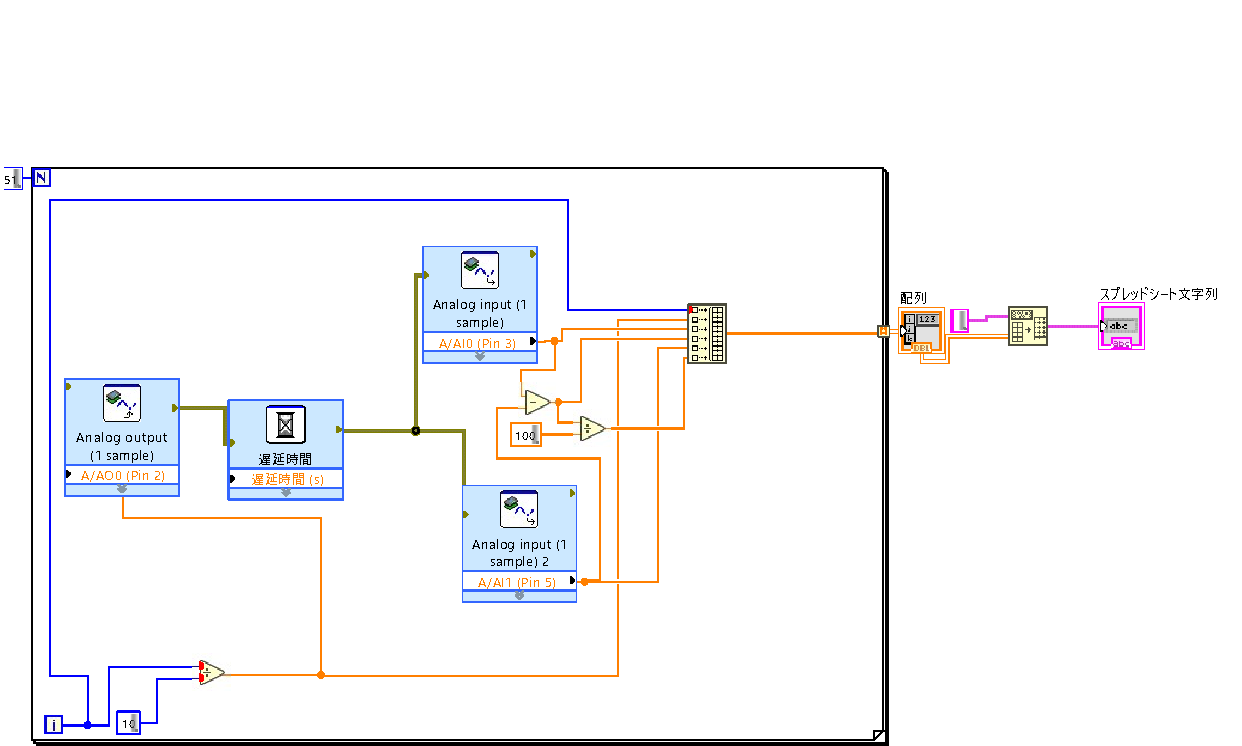
\includegraphics[scale=0.5]{./fig/ex31-block.pdf}\\
\useMycounter[\label{ex31-block}]固定抵抗の電圧電流特性計測時のブロックダイアグラム
\end{figure}
\begin{figure}[h]
\centering
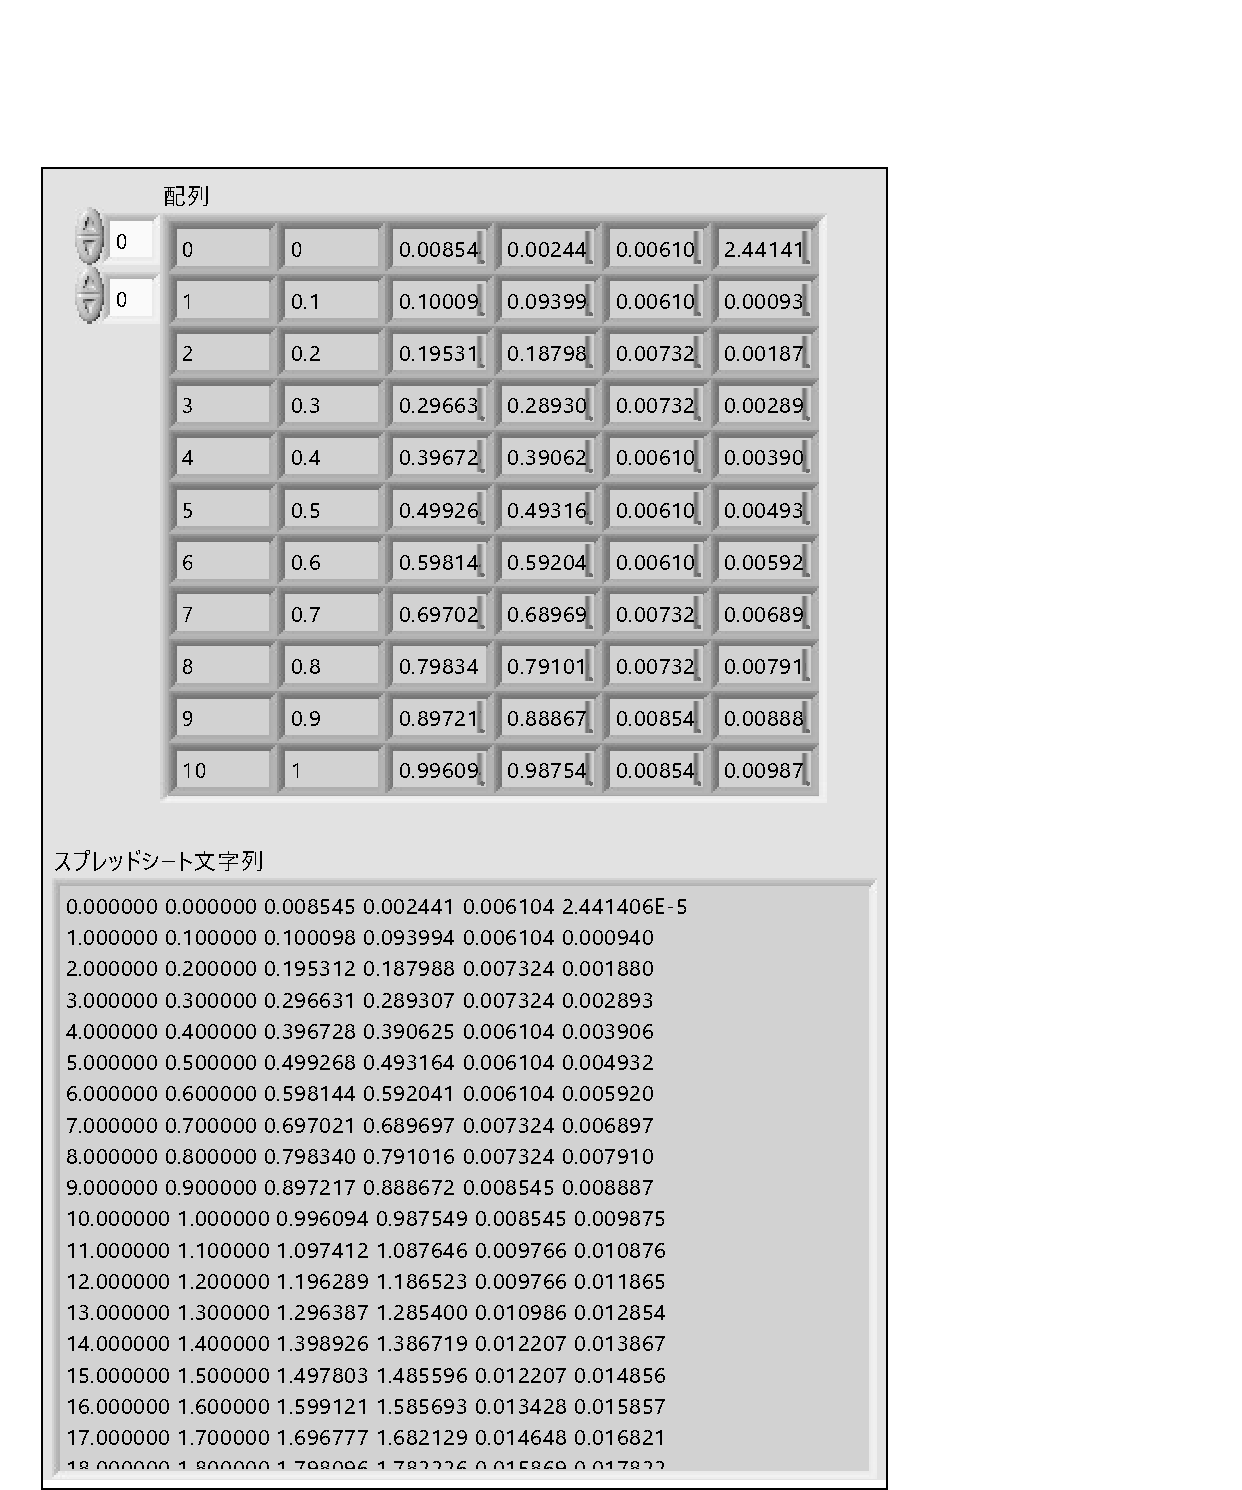
\includegraphics[scale=0.5]{./fig/ex31-flont.pdf}
\caption{固定抵抗の電圧電流特性測定時のフロントパネル}
\label{fig:ex31-flont}
\end{figure}

\begin{table}[h]
    \centering
     \caption{固定抵抗の諸特性値}    
     \label{tab:R}
     \scalebox{0.8}{
    \begin{tabular}{cccccc}
\hline
カウンタ変数 & 出力電圧[\rm{V}] & 全電圧[\rm{V}]  & $V_{R0}$[\rm{V}]   & $V_{U}$[\rm{V}]    & $I_{U}$[\rm{A}]  \\
\hline
  0      & 0    & 0.007324 & 0        & 0.007324 & 0        \\
  1      & 0.1  & 0.096436 & 0.007324 & 0.089111 & 0.0000732 \\
  2      & 0.2  & 0.197754 & 0.019531 & 0.178223 & 0.000195 \\
  3      & 0.3  & 0.297852 & 0.026855 & 0.270996 & 0.000269 \\
  4      & 0.4  & 0.39917  & 0.037842 & 0.361328 & 0.000378 \\
  5      & 0.5  & 0.498047 & 0.046387 & 0.45166  & 0.000464 \\
  6      & 0.6  & 0.595703 & 0.05249  & 0.543213 & 0.000525 \\
  7      & 0.7  & 0.697021 & 0.063477 & 0.633545 & 0.000635 \\
  8      & 0.8  & 0.797119 & 0.073242 & 0.723877 & 0.000732 \\
  9      & 0.9  & 0.897217 & 0.084229 & 0.812988 & 0.000842 \\
  10     & 1    & 0.996094 & 0.091553 & 0.904541 & 0.000916 \\
  11     & 1.1  & 1.096191 & 0.101318 & 0.994873 & 0.001013 \\
  12     & 1.2  & 1.195068 & 0.108643 & 1.086426 & 0.001086 \\
  13     & 1.3  & 1.297607 & 0.12207  & 1.175537 & 0.001221 \\
  14     & 1.4  & 1.396484 & 0.128174 & 1.26831  & 0.001282 \\
  15     & 1.5  & 1.496582 & 0.13916  & 1.357422 & 0.001392 \\
  16     & 1.6  & 1.5979   & 0.150146 & 1.447754 & 0.001501 \\
  17     & 1.7  & 1.696777 & 0.157471 & 1.539306 & 0.001575 \\
  18     & 1.8  & 1.795654 & 0.164795 & 1.630859 & 0.001648 \\
  19     & 1.9  & 1.895752 & 0.174561 & 1.721191 & 0.001746 \\
  20     & 2    & 1.994629 & 0.183105 & 1.811523 & 0.001831 \\
  21     & 2.1  & 2.094726 & 0.192871 & 1.901855 & 0.001929 \\
  22     & 2.2  & 2.194824 & 0.202637 & 1.992187 & 0.002026 \\
  23     & 2.3  & 2.294922 & 0.211182 & 2.08374  & 0.002112 \\
  24     & 2.4  & 2.395019 & 0.220947 & 2.174072 & 0.002209 \\
  25     & 2.5  & 2.495117 & 0.230713 & 2.264404 & 0.002307 \\
  26     & 2.6  & 2.593994 & 0.238037 & 2.355957 & 0.00238  \\
  27     & 2.7  & 2.694092 & 0.247803 & 2.446289 & 0.002478 \\
  28     & 2.8  & 2.794189 & 0.257568 & 2.536621 & 0.002576 \\
  29     & 2.9  & 2.894287 & 0.266113 & 2.628174 & 0.002661 \\
  30     & 3    & 2.995605 & 0.2771   & 2.718506 & 0.002771 \\
  31     & 3.1  & 3.094482 & 0.285645 & 2.808838 & 0.002856 \\
  32     & 3.2  & 3.193359 & 0.29541  & 2.897949 & 0.002954 \\
  33     & 3.3  & 3.293457 & 0.302734 & 2.990722 & 0.003027 \\
  34     & 3.4  & 3.393554 & 0.3125   & 3.081054 & 0.003125 \\
  35     & 3.5  & 3.492431 & 0.321045 & 3.171386 & 0.00321  \\
  36     & 3.6  & 3.59497  & 0.333252 & 3.261718 & 0.003333 \\
  37     & 3.7  & 3.693847 & 0.339355 & 3.354492 & 0.003394 \\
  38     & 3.8  & 3.793945 & 0.349121 & 3.444824 & 0.003491 \\
  39     & 3.9  & 3.894043 & 0.358887 & 3.535156 & 0.003589 \\
  40     & 4    & 3.99292  & 0.367432 & 3.625488 & 0.003674 \\
  41     & 4.1  & 4.091796 & 0.374756 & 3.717041 & 0.003748 \\
  42     & 4.2  & 4.193115 & 0.385742 & 3.807373 & 0.003857 \\
  43     & 4.3  & 4.274902 & 0.390625 & 3.884277 & 0.003906 \\
  44     & 4.4  & 4.272461 & 0.391846 & 3.880615 & 0.003918 \\
  45     & 4.5  & 4.270019 & 0.390625 & 3.879394 & 0.003906 \\
  46     & 4.6  & 4.268798 & 0.390625 & 3.878173 & 0.003906 \\
  47     & 4.7  & 4.266357 & 0.390625 & 3.875732 & 0.003906 \\
  48     & 4.8  & 4.266357 & 0.391846 & 3.874511 & 0.003918 \\
  49     & 4.9  & 4.263916 & 0.390625 & 3.873291 & 0.003906 \\
  50     & 5    & 4.262695 & 0.389404 & 3.873291 & 0.003894 \\
\hline
\end{tabular}
}
\end{table}

\begin{figure}[h]
        \centering
        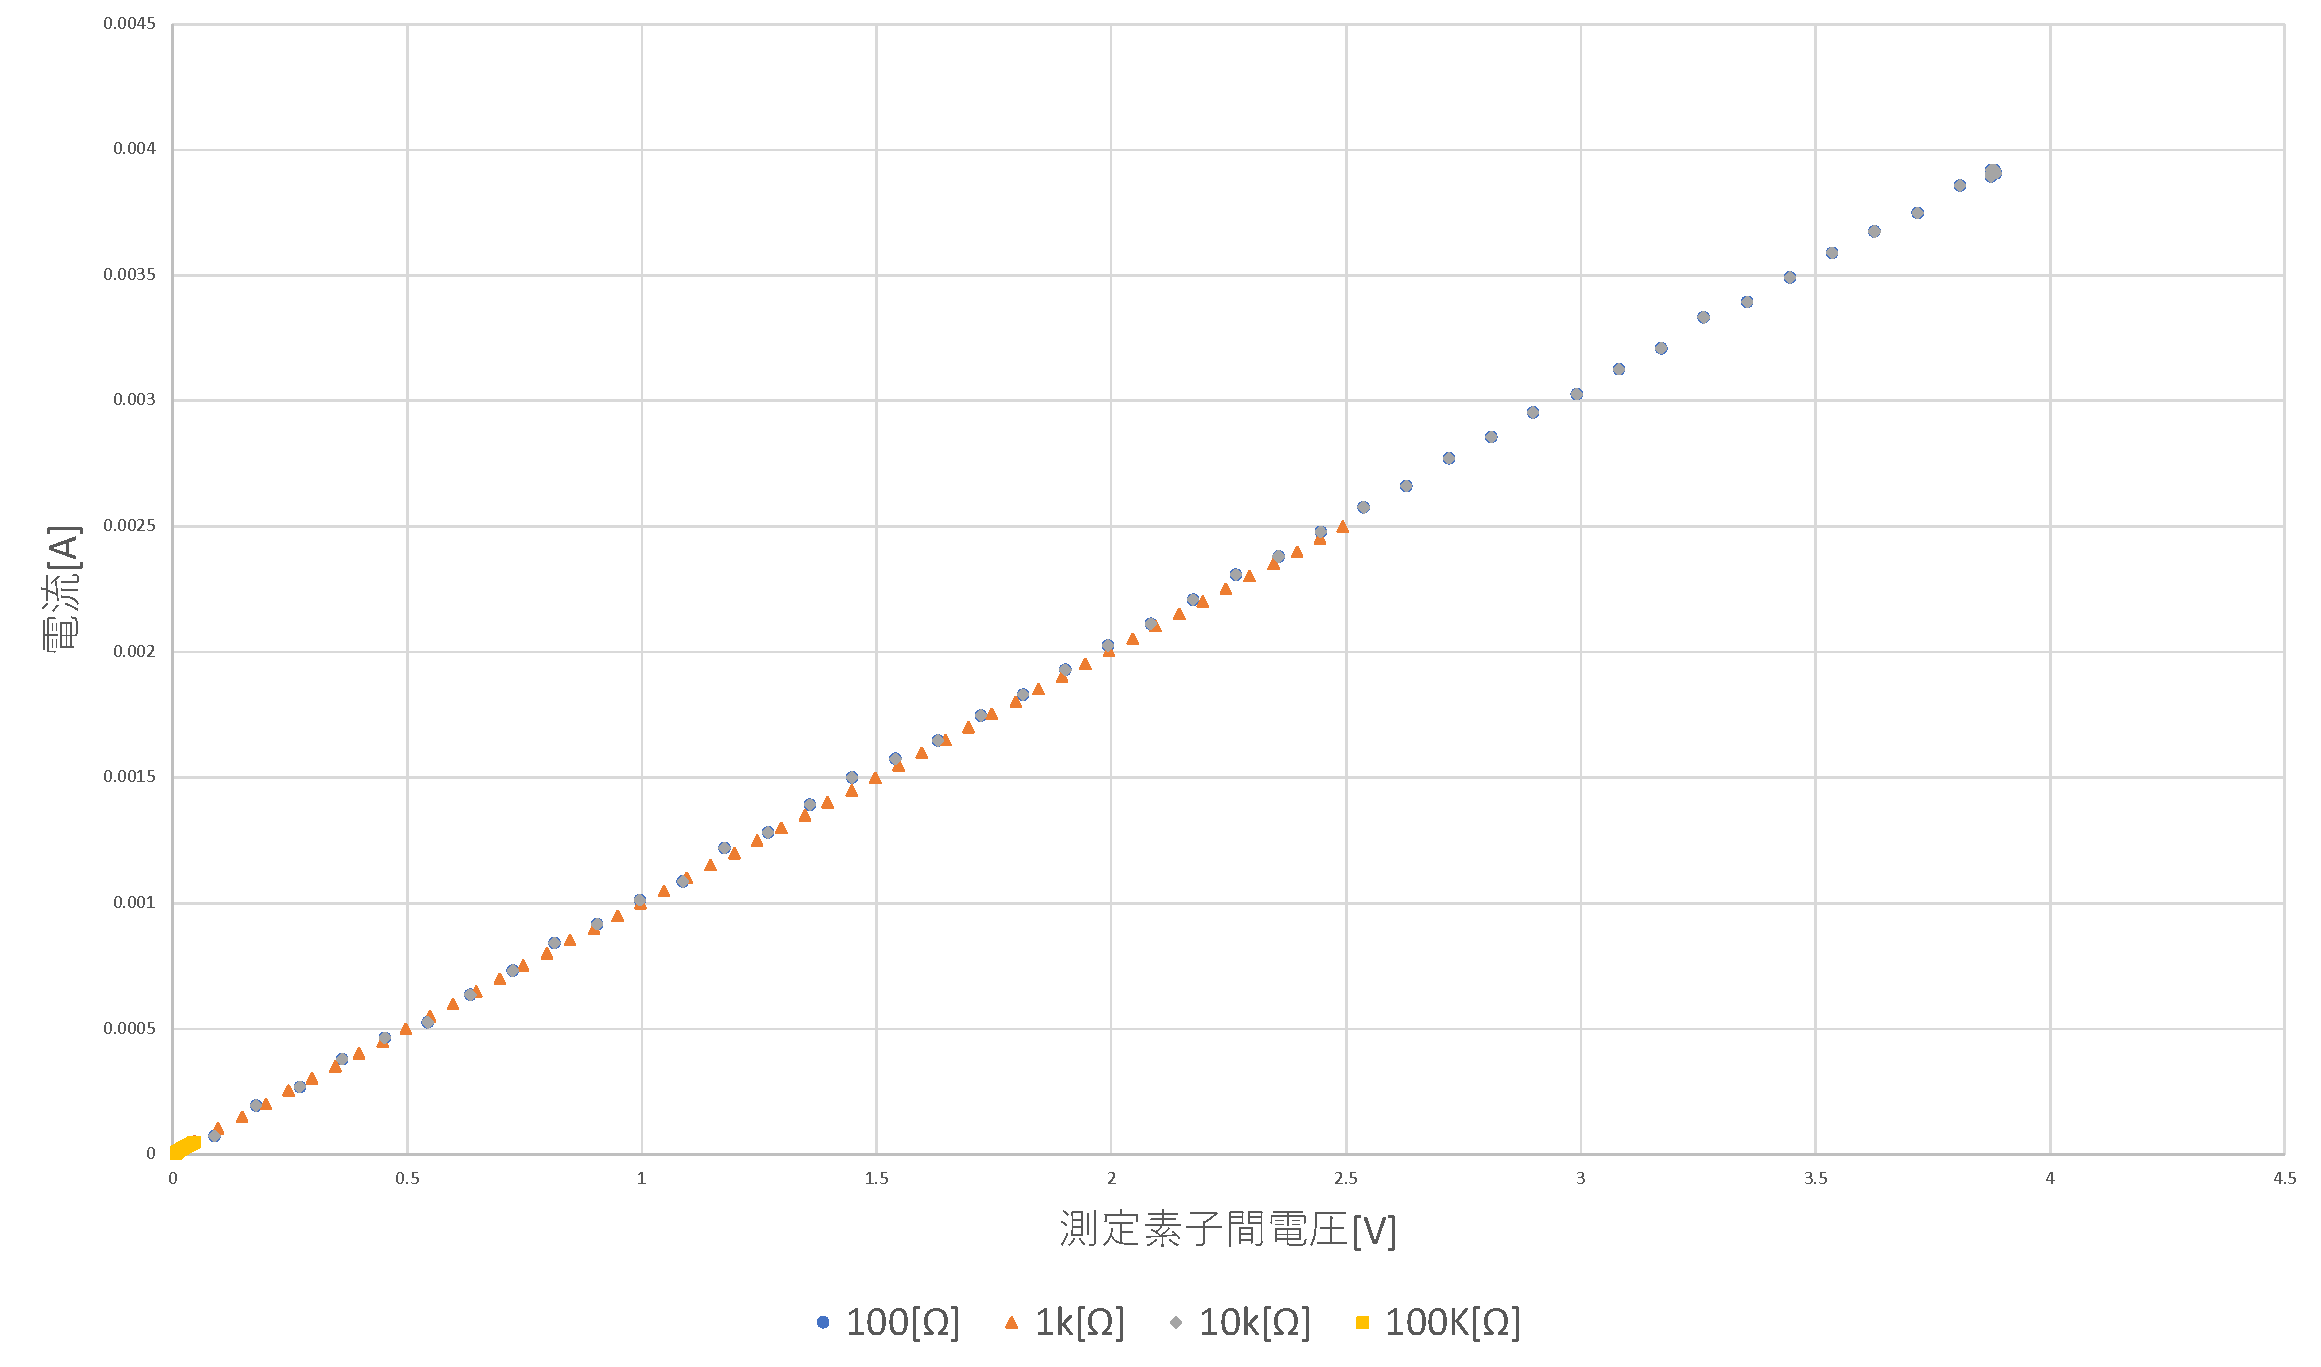
\includegraphics[scale=0.45]{./fig/3-1.pdf}
	\caption{固定抵抗の電圧電流特性}
	\label{fig:3-1}  
\end{figure}